\documentclass{beamer}
\usepackage{tikz,amsmath,amssymb,hyperref,graphicx,stackrel,setspace,animate}
\usetikzlibrary{positioning,shadows,arrows,shapes,calc}
\newcommand{\argmax}{\operatornamewithlimits{argmax}}
\newcommand{\argmin}{\operatornamewithlimits{argmin}}
\mode<presentation>{\usetheme{Frankfurt}}
\DeclareMathOperator*{\softmax}{softmax}
\AtBeginSection[]
{
  \begin{frame}<beamer>
    \frametitle{Outline}
    \tableofcontents[currentsection,currentsubsection]
  \end{frame}
}
\title{Lecture 9: Convolutional Neural Nets}
\author{Mark Hasegawa-Johnson\\These slides are in the public domain}
\date{ECE 417: Multimedia Signal Processing, Fall 2023}  
\begin{document}

% Title
\begin{frame}
  \maketitle
\end{frame}

% Title
\begin{frame}
  \tableofcontents
\end{frame}


%%%%%%%%%%%%%%%%%%%%%%%%%%%%%%%%%%%%%%%%%%%%
\section[Review]{Review: Neural Network}
\setcounter{subsection}{1}

\begin{frame}
  \frametitle{Review: How to train a neural network}
  \begin{enumerate}
  \item Find a {\bf training dataset} that contains $n$ examples showing the
    desired output, $\mathbf{y}_i$, that the NN should compute in
    response to input vector $\mathbf{x}_i$:
    \[
    {\mathcal D}=\left\{(\mathbf{x}_1,\mathbf{y}_1),\ldots,(\mathbf{x}_n,\mathbf{y}_n)\right\}
    \]
    \item Randomly {\bf initialize} the weights and biases, $\mathbf{W}_{1}$,
      $\mathbf{b}_{1}$, $\mathbf{W}_{2}$, and $\mathbf{b}_{2}$.
    \item Perform {\bf forward propagation}: find out what the neural
      net computes as $\mathbf{g}(\mathbf{x}_i)$ for each $\mathbf{x}_i$.
    \item Define a {\bf loss function} that measures
      how badly $\mathbf{g}(\mathbf{x})$ differs from $\mathbf{y}$.
    \item Perform {\bf back propagation} to improve $\mathbf{W}_{1}$,
      $\mathbf{b}_{1}$, $\mathbf{W}_{2}$, and $\mathbf{b}_{2}$.
    \item Repeat steps 3-5 until convergence.
  \end{enumerate}
\end{frame}

\begin{frame}
  \frametitle{Review: Second Layer = Piece-Wise Approximation}

  The second layer of the network approximates
  $\mathbf{g}(\mathbf{x})\approx\mathbf{y}$ using a bias term
  $\mathbf{b}$, plus correction vectors $\mathbf{w}_{2,:,j}$, each
  scaled by its activation $h_j$:
  \[
  \mathbf{g}(\mathbf{x}) = \mathbf{b}_{2} + \sum_j \mathbf{w}_{2,:,j} h_j
  \]
  \begin{itemize}
  \item Unit-step and signum nonlinearities, on the hidden layer,
    cause the neural net to compute a piece-wise constant approximation
    of the target function. Sigmoid and tanh are differentiable approximations of
    unit-step and signum, respectively.
  \item ReLU, Leaky ReLU, and PReLU activation functions cause $h_j$,
    and therefore $\mathbf{g}(\mathbf{x})$, to be a piece-wise-linear function of its
    inputs.
  \end{itemize}
\end{frame}

\begin{frame}
  \frametitle{Review: First Layer = A Series of Decisions}

  The first layer of the network decides whether or not to ``turn on'' each of the
  $h_j$'s.  It does this by comparing $\mathbf{x}$ to a series of linear threshold vectors:
  \[
  h_k = \sigma\left(\mathbf{w}_{1,k,:}^T\mathbf{x}+b_k\right)\begin{cases}
  \approx 1 & \mathbf{w}_{1,k,:}^T\mathbf{x} +b_k > 0\\
  \approx 0 & \mathbf{w}_{1,k,:}^T\mathbf{x} +b_k < 0
  \end{cases}
  \]
\end{frame}

\begin{frame}
  \frametitle{Gradient Descent: How do we improve $\mathbf{W}_l$ and $\mathbf{b}_l$?}  Given
  some initial neural net parameter, $w_{l,k,j}$, we want to
  find a better value of the same parameter.  We do that using
  gradient descent:
  \[
  w_{l,k,j} \leftarrow w_{l,k,j}-\eta\frac{d{\mathcal L}}{dw_{l,k,j}},
  \]
  where $\eta$ is a learning rate (some small constant, e.g., $\eta=0.001$ or so).
  \centerline{\includegraphics[width=2in]{exp/gradient_descent.png}}
\end{frame}

\begin{frame}
  \frametitle{Error Metrics Summarized}
  \begin{itemize}
    \item Use MSE to achieve $\mathbf{g}(\mathbf{x})\rightarrow
      E\left[\mathbf{y}|\mathbf{x}\right]$: appropriate for regression applications.
    \item For a binary classifier with a sigmoid output, BCE loss gives you
      the MSE result without the vanishing gradient problem.
    \item For a multi-class classifier with a softmax output, CE loss gives you
      the MSE result without the vanishing gradient problem.
    \item After you're done training, you can make your cell phone app
      more efficient by throwing away the uncertainty:
      \begin{itemize}
      \item Replace softmax output nodes with max
      \item Replace logistic output nodes with unit-step
      \item Replace tanh output nodes with signum
      \end{itemize}
  \end{itemize}
\end{frame}

%%%%%%%%%%%%%%%%%%%%%%%%%%%%%%%%%%%%%%%%%%%%
\section[Convolution]{Convolutional Layers}
\setcounter{subsection}{1}

\begin{frame}
  \frametitle{Multimedia Inputs = Too Much Data}
  \begin{columns}[t]
    \column{1in}
    \begin{block}{}
      \centerline{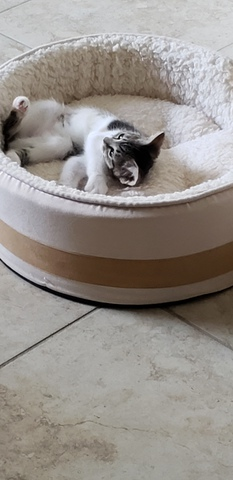
\includegraphics[width=0.8in]{figs/kitten.jpg}}
    \end{block}
    \column{3.5in}
    \begin{block}{Does this image contain a  cat?}
      Fully-connected solution:
      \begin{align*}
        \mathbf{g}(\mathbf{x}) &=\sigma\left(\mathbf{W}_{2}\mathbf{a}_1+\mathbf{b}_2\right)\\
        \mathbf{a}_1 &= \mbox{ReLU}\left(\mathbf{W}_{1}\mathbf{x}+\mathbf{b}_1\right)
      \end{align*}
      where $\mathbf{x}$ contains all the pixels.
      \begin{itemize}
      \item Image size $2000\times 3000\times 3=18,000,000$ dimensions in $\mathbf{x}$.
      \item If $\mathbf{a}_1$ has 500 dimensions, then $\mathbf{W}_{1}$ has
        $500\times 18,000,000=9,000,000,000$ parameters.
      \item \ldots so we should use at least $9,000,000,000$ images to train it.
      \end{itemize}
    \end{block}
  \end{columns}
\end{frame}

\begin{frame}
  \frametitle{Shift Invariance}
  \centerline{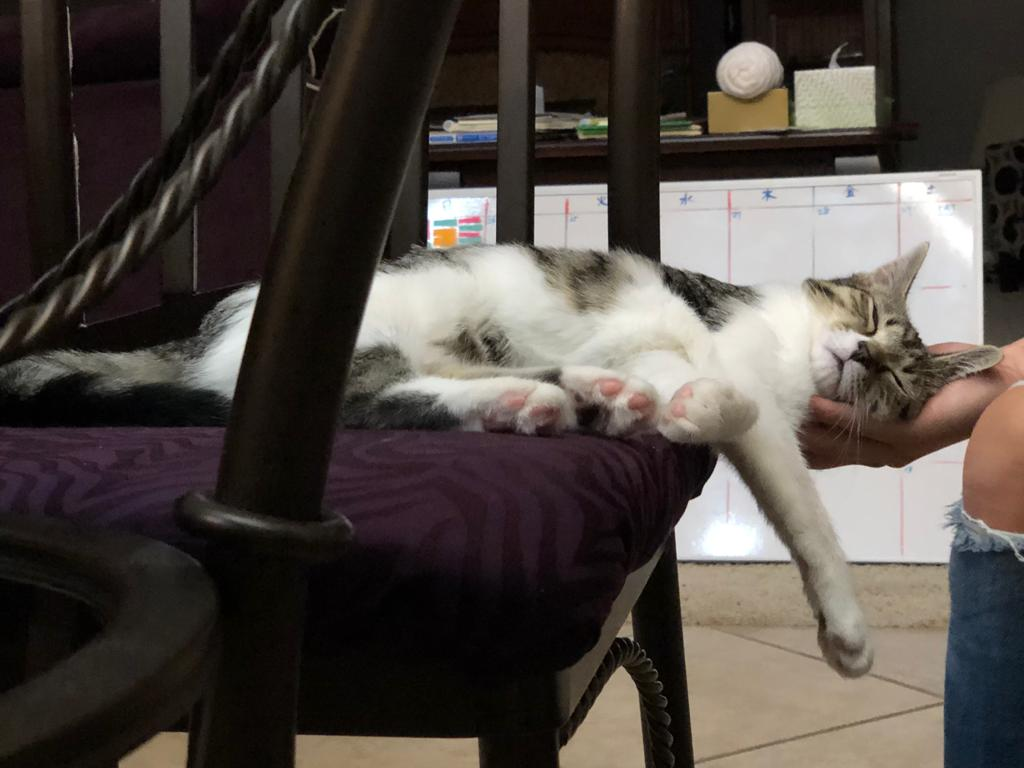
\includegraphics[height=1.5in]{figs/IMG-20200826-WA0000.jpg}}
    The cat has moved.  The fully-connected network has no way to
    share information between the rows of $\mathbf{W}_{1}$ that look at the
    center of the image, and the rows that look at the right-hand side.
\end{frame}

\begin{frame}
  \frametitle{How to achieve shift invariance: Convolution}

  Instead of using vectors as layers, let's use images.
  \begin{align*}
    z[l,d,m,n] &= \sum_c\sum_{m'}\sum_{n'} w[l,d,c,m-m',n-n']a[l-1,c,m',n']
  \end{align*}
  where
  \begin{itemize}
  \item $z[l,c,m,n]$ and $a[l,c,m,n]$ are excitation and
    activation (respectively) of the $(m,n)^{\textrm{th}}$ pixel, in
    the $c^{\textrm{th}}$ channel, in the $l^{\textrm{th}}$ layer.
  \item $w[l,d,c,m-m',n-n']$ are weights connecting $c^{\textrm{th}}$
    input channel to $d^{\textrm{th}}$ output channel, with a shift of
    $m-m'$ rows, $n-n'$ columns.
  \end{itemize}
\end{frame}

\begin{frame}
  \frametitle{How to achieve shift invariance: Convolution}

  \centerline{\animategraphics[loop,controls,width=0.8\textwidth]{20}{exp/forward}{0}{99}}
\end{frame}

\begin{frame}
  \frametitle{How to use convolutions in a classifier}
  \begin{itemize}
  \item The zero$^{\textrm{th}}$ layer is the input image, where
    $c\in\left\{1,2,3\right\}$ denotes color (red, green or blue):
    \[
    a[0,c,m,n] = x[c,m,n]
    \]
  \item Excitation and activation:
    \begin{align*}
      z[l,d,m,n] &= \sum_c\sum_{m'}\sum_{n'} w[d,c,m-m',n-n']a[l-1,c,m',n']\\
      a[l,d,m,n] &= \mbox{ReLU}\left(z[l,d,m,n]\right)
    \end{align*}
  \item Reshape the last convolutional layer into a vector, to form
    the first fully-connected layer:
    \[
    \mathbf{a}_{L+1}=[a[L,1,1,1], a[L,1,1,2],\ldots, a[L,3,M,N]]^T
    \]
    where $M\times N$ is the image dimension.
  \end{itemize}
\end{frame}
      
\begin{frame}
  \frametitle{How to use convolutions in a classifier}

  \centerline{\includegraphics[width=4.5in]{exp/800px-Typical_cnn.png}}
  \begin{tiny}
    ``Typical CNN,'' by Aphex34 2015, CC-SA 4.0,
    \url{https://commons.wikimedia.org/wiki/File:Typical_cnn.png}
  \end{tiny}
\end{frame}

%%%%%%%%%%%%%%%%%%%%%%%%%%%%%%%%%%%%%%%%%%%%
\section[Backprop]{Backprop of Convolution is Correlation}
\setcounter{subsection}{1}

\begin{frame}
  \frametitle{How to back-prop through a convolutional neural net}

  You already know how to back-prop through fully-connected layers.  Now let's
  back-prop through convolution:
  \begin{displaymath}
    \frac{\partial{\mathcal L}}{\partial a[l-1,c,m',n']} =
    \sum_{m}\sum_n\sum_d\frac{\partial{\mathcal L}}{\partial z[l,d,m,n]}
    \frac{\partial z[l,d,m,n]}{\partial a[l-1,c,m',n']}
  \end{displaymath}
  We need to find two things:
  \begin{enumerate}
  \item What is $\frac{\partial{\mathcal L}}{\partial z[l,d,m,n]}$?
    Answer: We can assume it's already known, because we have already back-propagated as
    far as layer $l$.
  \item What is $\frac{\partial z[l,d,m,n]}{\partial a[l-1,c,m',n']}$?
    Answer: That is the new thing that we need, in orer to back-propagate to
    layer $l-1$.
  \end{enumerate}
\end{frame}

\begin{frame}
  \frametitle{How to back-prop through convolution}

  Here is the formula for convolution:
  \begin{align*}
    z[l,d,m,n] &= \sum_c\sum_{m'}\sum_{n'} w[l,d,c,m-m',n-n']a[l-1,c,m',n']
  \end{align*}
  If we differentiate the left side w.r.t. the right side, we get:
  \begin{align*}
    \frac{\partial z[l,d,m,n]}{\partial a[l-1,c,m',n']} &= w[l,d,c,m-m',n-n']
  \end{align*}
  Plugging into the formula on the previous slide, we get:
  \begin{displaymath}
    \frac{\partial{\mathcal L}}{\partial a[l-1,c,m',n']} =
    \sum_{m}\sum_n\sum_d w[l,d,c,m-m',n-n']\frac{d{\mathcal L}}{dz[l,d,m,n]}
  \end{displaymath}
\end{frame}

\begin{frame}
  \frametitle{Convolution forward, Correlation backward}

  In signal processing, we defined $a[n]\ast w[n]$ to mean $\sum
  w[n']a[n-n']$.  Let's use the same symbol to refer to this
  multi-channel 2D convolution:
  \begin{align*}
    z[l,d,m,n] &= \sum_c\sum_{m'}\sum_{n'} w[l,d,c,m-m',n-n']a[l-1,c,m',n']\\
    &\equiv w[l,m,n,c,d] \ast h[l-1,c,m,n]
  \end{align*}
  Back-propagation looks kind of similar, but notice that now, instead
  of $\sum_{n'}w[n-n']a[n']$, we have $\sum_nw[n-n']a[n]$:
  \begin{align*}
    \frac{\partial{\mathcal L}}{\partial a[l-1,c,m',n']} &=
    \sum_{m}\sum_{n}\sum_c w[l,d,c,m-m',n-n']\frac{\partial{\mathcal L}}{\partial z[l,d,m,n]}
  \end{align*}
  In other words, we are summing over the variable on which $w[n]$ has
  {\bf not been flipped}.  What is that?
\end{frame}

\begin{frame}
  \frametitle{Convolution versus Correlation}
  \centerline{\includegraphics[width=0.8\textwidth]{exp/convolution_correlation.png}}
  \url{https://upload.wikimedia.org/wikipedia/commons/thumb/2/21/Comparison_convolution_correlation.svg/1024px-Comparison_convolution_correlation.svg.png}
\end{frame}

\begin{frame}
  \frametitle{Convolution versus Correlation}
  \begin{itemize}
  \item Convolution is when we flip one of the two signals, shift, multiply, then add:
    \begin{displaymath}
      a[m]\ast w[m] = \sum_{m'} w[m-m']a[m']
    \end{displaymath}
  \item Correlation is when we only shift, multiply, and add:
    \begin{displaymath}
      a[m']\bigstar w[m'] = \sum_m w[m-m']a[m]
    \end{displaymath}
  \end{itemize}
\end{frame}

\begin{frame}
  \frametitle{The Back-Prop of Convolution is Correlation}

  \begin{align*}
    \frac{\partial{\mathcal L}}{\partial a[l-1,c,m',n']} &=
    \sum_{m}\sum_{n}\sum_c w[l,d,c,m-m',n-n']\frac{\partial{\mathcal L}}{\partial z[l,d,m,n]}\\
    &= w[l,d,c,m',n'] \bigstar \frac{d{\mathcal L}}{\partial z[l,d,m',n']}
  \end{align*}
\end{frame}

\begin{frame}
  \frametitle{The Back-Prop of Convolution is Correlation}

  \begin{align*}
    z[l,d,m,n] &= w[l,m,n,c,d] \ast h[l-1,c,m,n]
  \end{align*}
  \begin{align*}
    \frac{\partial{\mathcal L}}{\partial a[l-1,c,m',n']}
    &= w[l,d,c,m',n'] \bigstar \frac{d{\mathcal L}}{\partial z[l,d,m',n']} 
  \end{align*}
\end{frame}


\begin{frame}
  \frametitle{Back-prop through a convolutional layer}

  \centerline{\animategraphics[loop,controls,width=0.8\textwidth]{20}{exp/backward}{0}{74}}
\end{frame}

\begin{frame}
  \frametitle{Similarities between convolutional and fully-connected back-prop}

  \begin{itemize}
  \item In a fully-connected layer, forward-prop means multiplying a
    matrix by a column vector on the right.  Back-prop means
    multiplying the same matrix by a row vector from the left:
    \begin{align*}
      \mathbf{z}_{l} &= \mathbf{W}_l\mathbf{a}_{l-1}\\
      \frac{\partial\mathcal{L}}{\partial\mathbf{a}_{l-1}}
      &= \frac{\partial\mathcal{L}}{\partial\mathbf{z}_{l}}\mathbf{W}_l
    \end{align*}
  \item In a convolutional layer, forward-prop is a convolution,
    Back-prop is a correlation:
    \begin{align*}
    z[l,d,m,n] &= w[l,m,n,c,d] \ast h[l-1,c,m,n]\\
    \frac{d{\mathcal L}}{dh[l-1,c,m,n]} &=
    w[l,d,c,m',n'] \bigstar \frac{d{\mathcal L}}{dz[l,d,m',n']}\\
    \end{align*}
  \end{itemize}
\end{frame}
    
\begin{frame}
  \frametitle{Convolutional layers: Weight gradient}

  Finally, we need to combine back-prop and forward-prop in order to
  find  the weight gradient:
  \begin{align*}
    \frac{d{\mathcal L}}{dw[l,d,c,m',n']} &=
    \sum_{m}\sum_n\frac{d{\mathcal L}}{dz[l,d,m,n]}
    \frac{\partial z[l,d,m,n]}{\partial w[l,d,c,m',n']}
  \end{align*}
  Again, here's the formula for convolution:
  \begin{align*}
    z[l,d,m,n] &= \sum_c\sum_{m'}\sum_{n'} w[l,d,c,m',n']a[l-1,c,m-m',n-n']
  \end{align*}
  If we differentiate the left side w.r.t. the right side, we get:
  \begin{align*}
    \frac{\partial z[l,d,m,n]}{\partial w[l,d,c,m',n']} &= a[l-1,c,m-m',n-n']
  \end{align*}
\end{frame}

\begin{frame}
  \frametitle{Convolutional layers: Weight gradient}

  \begin{align*}
    \frac{\partial{\mathcal L}}{\partial w[l,d,c,m',n']} &=
    \sum_{m}\sum_n\frac{d{\mathcal L}}{dz[l,d,m,n]}
    \frac{\partial z[l,d,m,n]}{\partial w[l,d,c,m',n']}
  \end{align*}
  \begin{align*}
    \frac{\partial z[l,d,m,n]}{\partial w[l,d,c,m',n']} &= a[l-1,c,m-m',n-n']
  \end{align*}
  Putting those together, we discover that the weight gradient is a correlation:
  \begin{align*}
    \frac{\partial{\mathcal L}}{\partial w[l,d,c,m',n']} &=
    \sum_{m}\sum_n \frac{\partial{\mathcal L}}{\partial z[l,d,m,n]}a[l-1,c,m-m',n-n']\\
    &= \frac{\partial{\mathcal L}}{\partial z[l,d,m',n']} \bigstar a[l-1,c,m',n']
  \end{align*}
\end{frame}

\begin{frame}
  \frametitle{Steps in training a CNN}
  \begin{enumerate}
  \item Forward-prop is convolution:
    \begin{align*}
      z[l,d,m,n] &= w[l,d,c,m,n] \ast a[l-1,c,m,n]
    \end{align*}
  \item Back-prop is correlation:
    \begin{align*}
      \frac{\partial{\mathcal L}}{\partial a[l-1,c,m,n]} &=
      w[l,d,c,m,n] \bigstar \frac{\partial{\mathcal L}}{\partial z[l,d,m,n]}
    \end{align*}
  \item Weight gradient is correlation:
    \begin{align*}
      \frac{\partial{\mathcal L}}{\partial w[l,d,c,m,n]} &=
      \frac{\partial{\mathcal L}}{\partial z[l,d,m,n]} \bigstar a[l-1,c,m,n]
    \end{align*}
  \end{enumerate}
\end{frame}

%%%%%%%%%%%%%%%%%%%%%%%%%%%%%%%%%%%%%%%%%%%%%%%%%%%%%%%%%%%%%%%%%%%%%%
\section{Max Pooling}
\setcounter{subsection}{1}

\begin{frame}
  \frametitle{Features and PWL Functions}

  Remember the PWL model of a ReLU neural net:
  \begin{enumerate}
  \item The hidden layer activations are positive if some feature is
    detected in the input, and zero otherwise.
  \item The rows of the output layer are vectors, scaled by the hidden
    layer activations, in order to approximate some desired
    piece-wise-linear (PWL) output function.
  \item What happens next is different for regression and
    classification:
    \begin{enumerate}
    \item Regression: The PWL output function is the desired output.
    \item Classification: The PWL function is squashed down to the
      $[0,1]$ range using a sigmoid.
    \end{enumerate}
  \end{enumerate}
\end{frame}
       
\begin{frame}
  \frametitle{Features and PWL Functions}

  In image processing, often we don't care where in the image the
  ``feature'' occurs:
  \centerline{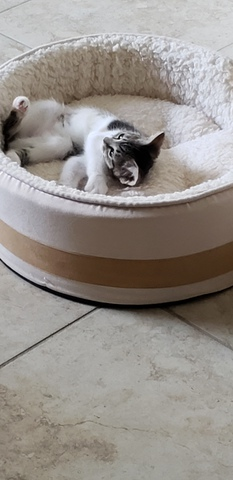
\includegraphics[height=2in]{figs/kitten.jpg}\hspace*{1cm}
    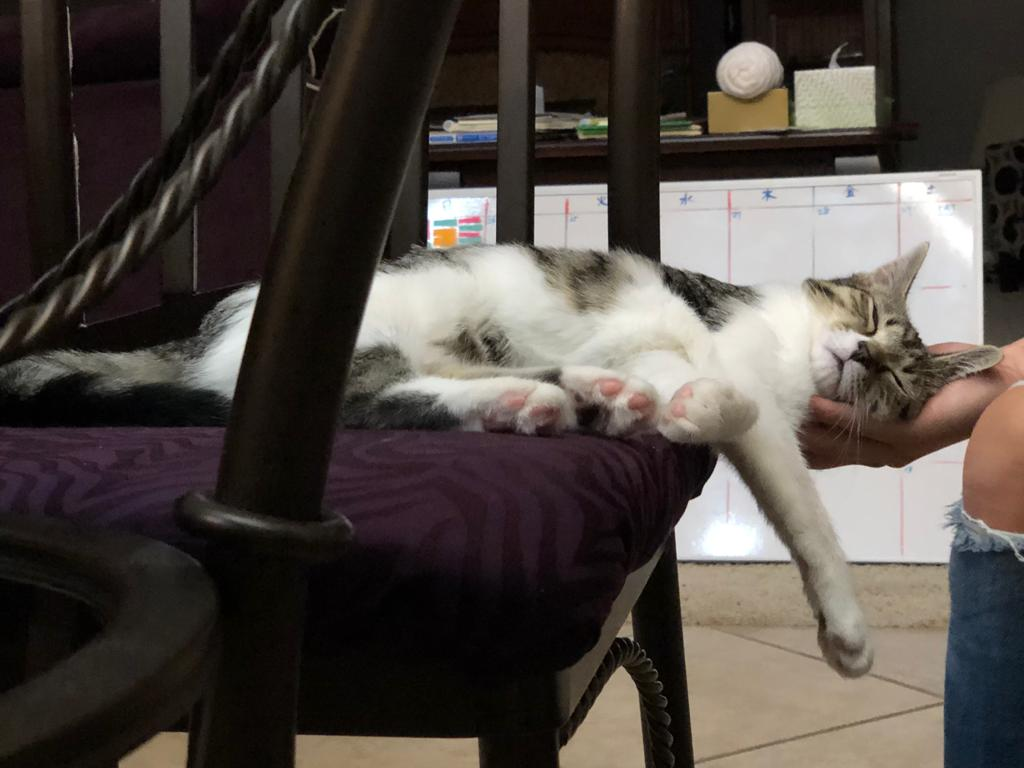
\includegraphics[height=2in]{figs/IMG-20200826-WA0000.jpg}}
\end{frame}

\begin{frame}
  \frametitle{Features and PWL Functions}

  Sometimes we care {\bf\em roughly} where the feature occurs, but not
  exactly.  Blue at the bottom is sea, blue at the top is sky:
  \centerline{\includegraphics[height=1.5in]{exp/Paracas.jpg}\hspace*{2mm}\includegraphics[height=1.5in]{exp/450px-Sky-3.jpg}}
  \begin{tiny}
    ``Paracas National Reserve,'' World Wide Gifts, 2011, CC-SA 2.0,
    \url{https://commons.wikimedia.org/wiki/File:Paracas_National_Reserve,_Ica,_Peru-3April2011.jpg}.
    ``Clouds above Earth at 10,000 feet,'' Jessie Eastland, 2010, CC-SA 4.0,
    \url{https://commons.wikimedia.org/wiki/File:Sky-3.jpg}.
  \end{tiny}
\end{frame}

\begin{frame}
  \frametitle{Max Pooling}
  \begin{itemize}
  \item Philosophy: the activation $a[l,c,m,n]$ should be greater
    than zero if the corresponding feature is detected anywhere within
    the vicinity of pixel $(m,n)$.  In fact, let's look for the {\em
      best matching} input pixel.
  \item Equation:
    \begin{displaymath}
      a[l,c,m,n] = \max_{m'=0}^{M-1}\max_{n'=0}^{M-1} \mbox{ReLU}\left(z[l,c,mM+m',nM+n']\right)
    \end{displaymath}
    where $M$ is a max-pooling factor (often $M=2$, but not always).
  \end{itemize}
\end{frame}

\begin{frame}
  \frametitle{Max Pooling}
  \centerline{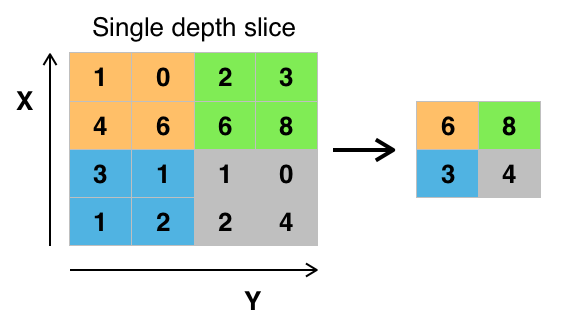
\includegraphics[height=2in]{exp/Max_pooling.png}}
  \begin{tiny}
    ``max pooling with 2x2 filter and stride = 2,'' Aphex34, 2015, CC SA 4.0,
    \url{https://commons.wikimedia.org/wiki/File:Max_pooling.png}
  \end{tiny}
\end{frame}

\begin{frame}
  \frametitle{Back-Prop for Max Pooling}

  The back-prop is pretty easy to understand.  The activation gradient,
  $\frac{\partial{\mathcal L}}{\partial a[l,c,m,n]}$, is back-propagated to just one of
  the excitation gradients in its pool: the one that had the maximum value.
  \begin{displaymath}
  \frac{\partial{\mathcal L}}{\partial z[l,c,mM+m',nM+n']}=
  \begin{cases}
    \frac{\partial{\mathcal L}}{\partial a[l,c,m,n]}
    & \begin{array}{l}(m',n')=(m^*,n^*)\\a[l,c,m,n]>0\end{array}\\
    0 & \mbox{otherwise},
  \end{cases}
  \end{displaymath}
  where:
  \begin{displaymath}
    (m^*,n^*)=\argmax_{m'=0}^{M-1}\argmax_{n'=0}^{M-1}z[l,c,mM+m',nM+n']
  \end{displaymath}
\end{frame}

\begin{frame}
  \frametitle{Other types of pooling}
  \begin{itemize}
  \item {\bf Average pooling:}
    \begin{displaymath}
      a[l,c,m,n] = \frac{1}{M^2}\sum_{m'=0}^{M-1}\sum_{n'=0}^{M-1} \mbox{ReLU}\left(z[l,c,mM+m',nM+n']\right)
    \end{displaymath}
    Philosophy: instead of finding the pixels that best match the feature,
    find the average degree of match.
%  \item {\bf Lp pooling:}
%    \begin{displaymath}
%      a[l,c,m,n] =
%      \left(\frac{1}{M^2}\sum_{m'=0}^{M-1}\sum_{n'=0}^{M-1} \mbox{ReLU}^{p}\left(z[l,c,mM+m',nM+n']\right)\right)^{1/p}
%    \end{displaymath}
%    Philosophy: Equals average pooling for $p=1$, approaches max pooling for $p\rightarrow\infty$.
  \item {\bf Decimation pooling:}
    \begin{displaymath}
      a[l,c,m,n] = \mbox{ReLU}\left(z[l,c,mM,nM]\right)
    \end{displaymath}
    Philosophy: the convolution has already done the averaging for you, so
    it's OK to just  throw away the other $M^2-1$ inputs.
  \end{itemize}
\end{frame}

%%%%%%%%%%%%%%%%%%%%%%%%%%%%%%%%%%%%%%%%%%%%%%%%%%%%%%%%%%%%%%%%%%%%%%
\section[Papers]{A Few Important Papers}
\setcounter{subsection}{1}

\begin{frame}
  \begin{columns}
    \column{2in}
    \begin{block}{``Phone Recognition: Neural Networks vs.~Hidden Markov Models,'' Waibel, Hanazawa,
        Hinton, Shikano and Lang, 1988}
      \begin{itemize}
      \item 1D convolution
      \item average pooling
      \item max pooling invented by Yamaguchi et  al., 1990, based on this architecture
      \end{itemize}
      \begin{tiny}
        {\setstretch{0.5}
          Image copyright Waibel et al., 1988, released CC-BY-4.0 2018,
          \url{https://commons.wikimedia.org/wiki/File:TDNN_Diagram.png}
          
        }
      \end{tiny}
    \end{block}
    \column{2in}
    \begin{block}{}
      \centerline{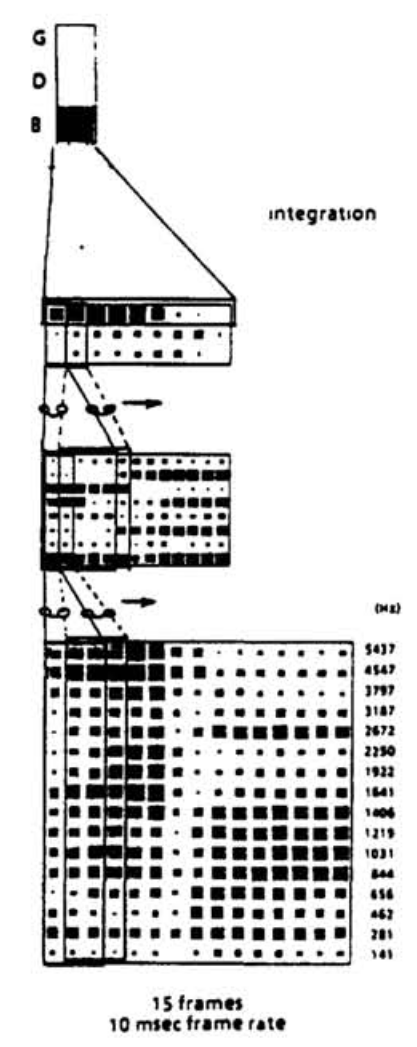
\includegraphics[height=3in]{figs/waibel1989.png}}
    \end{block}
  \end{columns}
\end{frame}

\begin{frame}
  \frametitle{``Backpropagation Applied to Handwritten Zip Code
    Recognition,'' LeCun, Boser, Denker \& Henderson, 1989 (2D
    convolution, decimation pooling)}
  \centerline{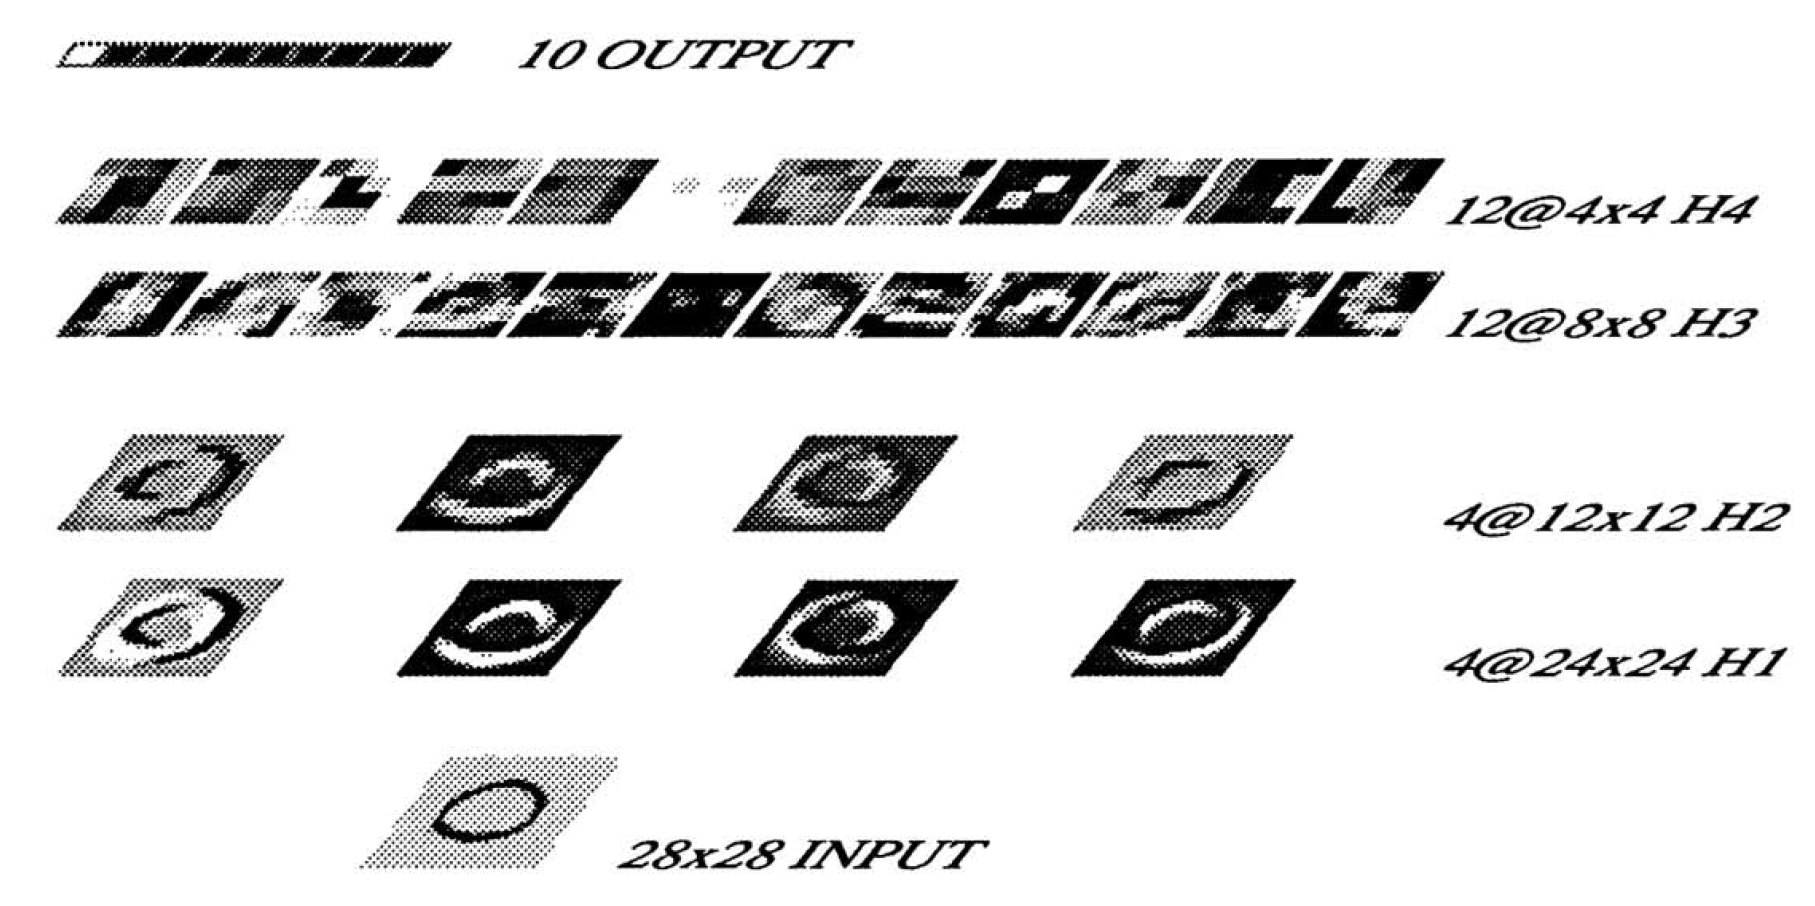
\includegraphics[width=4.5in]{figs/lecun1990.png}}
  \begin{tiny}Image copyright Lecun, Boser, et al., 1990\end{tiny}
\end{frame}

\begin{frame}
  \frametitle{``Imagenet Classification with Deep Convolutional Neural
    Networks,'' Krizhevsky, Sutskever \& Hinton, 2012 (GPU training)}
  \centerline{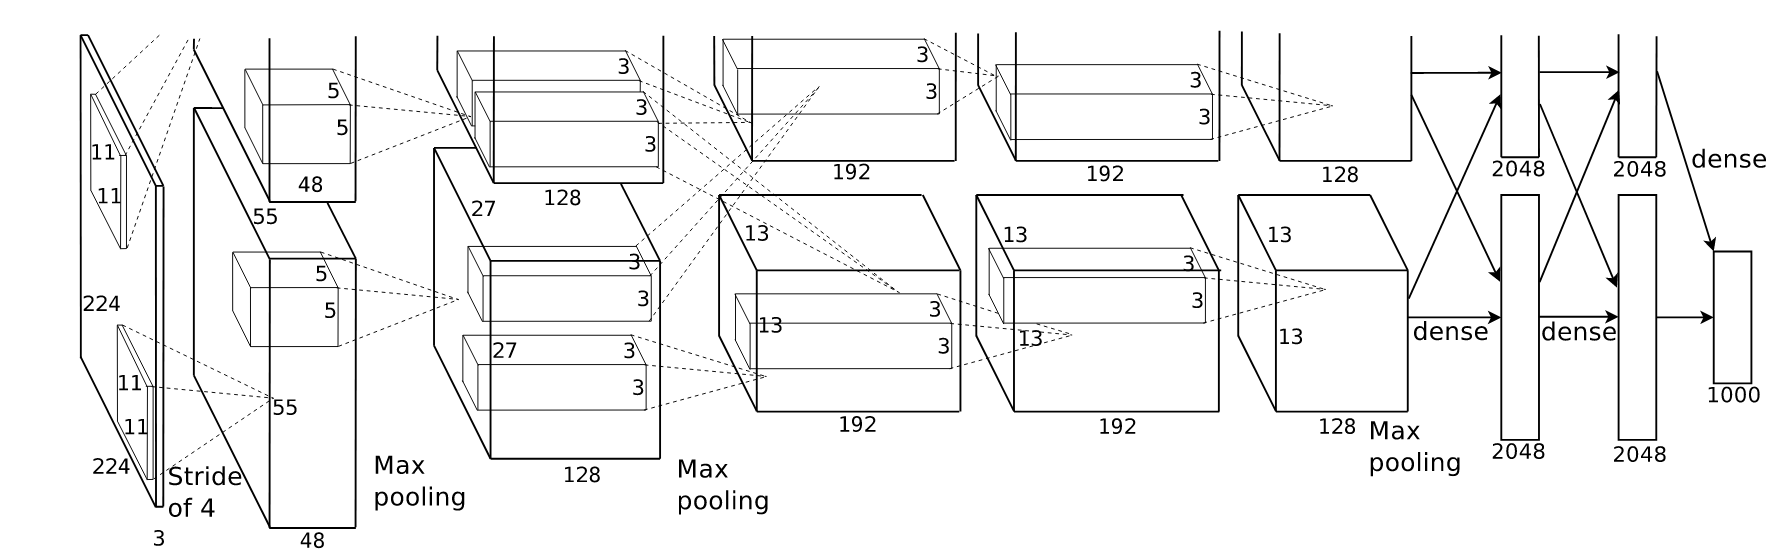
\includegraphics[width=4.75in]{figs/krizhevsky2012.png}}
  \begin{tiny}Image copyright Krizhevsky, Sutskever \& Hinton, 2012\end{tiny}
\end{frame}


%%%%%%%%%%%%%%%%%%%%%%%%%%%%%%%%%%%%%%%%%%%%%%%%%%%%%%%%%%%%%%%%%%%%%%
\section{Summary}
\setcounter{subsection}{1}

\begin{frame}
  \frametitle{Summary}
  \begin{itemize}
  \item Convolutional layers: forward-prop is a convolution, back-prop
    is a correlation, weight gradient is a correlation.
  \item Max pooling: back-prop just propagates the derivative to the
    pixel that was chosen by forward-prop.
  \item Many-layer CNNs trained on GPUs, with small convolutions in
    each layer, have won Imagenet every year since 2012, and are now a
    component in every image, speech, audio, and video processing
    system.
  \end{itemize}
\end{frame}

%%%%%%%%%%%%%%%%%%%%%%%%%%%%%%%%%%%%%%%%%%%%%%%%%%%%%%%%%%%%%%%%%%%%%%
\section[Example]{Written Example}
\setcounter{subsection}{1}

\begin{frame}
  \frametitle{Written Example}
  Suppose our input image is a delta function:
  \begin{displaymath}
    x[n] = \delta[n]
  \end{displaymath}
  Suppose we have one convolutional layer, and the weights are
  initialized to be Gaussian:
  \begin{displaymath}
    w[n] = e^{-\frac{n^2}{2}}
  \end{displaymath}
  Suppose that the neural net output is
  \begin{displaymath}
    \mathbf{g}(\mathbf{x})=\sigma\left(\max\left(w[n]\ast x[n]\right)\right),
  \end{displaymath}
  where $\sigma(\cdot)$ is the logistic sigmoid, and $\max(\cdot)$ is
  max-pooling over the entire output of the convolution.  Suppose that
  the target output is $y=1$, and we are using binary cross-entropy
  loss.  What is $d{\mathcal L}/dw[n]$, as a function of $n$?
\end{frame}

\end{document}

